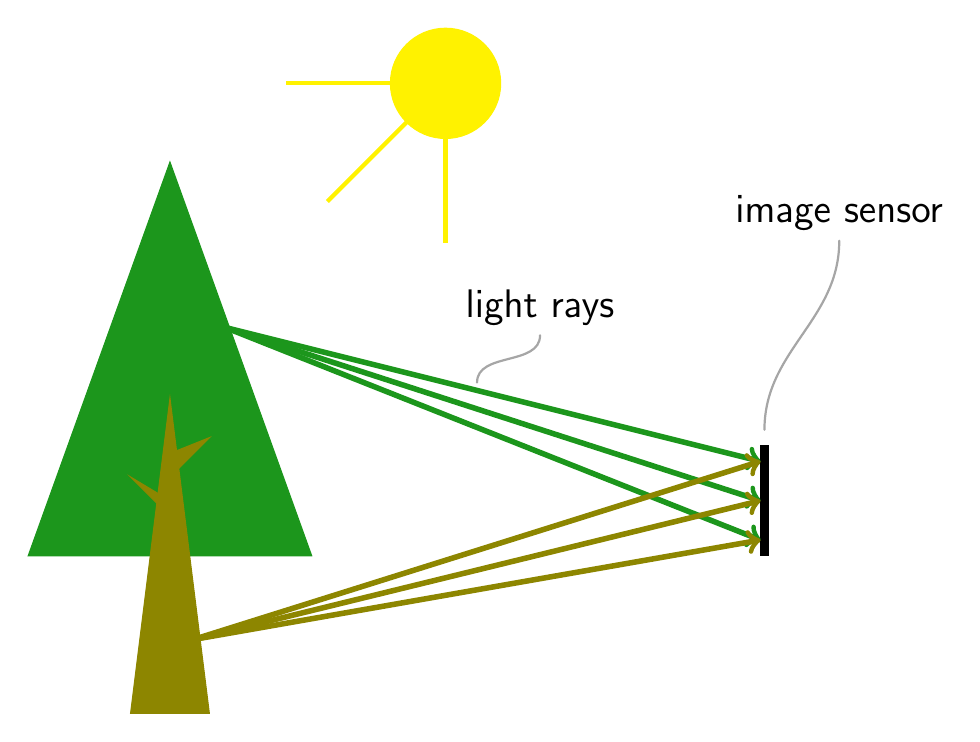
\begin{tikzpicture}  [
    description/.style={draw=gray!70, thick, line cap=round, every node/.style={align=center, font=\scriptsize\sffamily, anchor=north}},
  ]

\definecolor{mygreen}{RGB}{28, 150, 28}
%tree
%\draw[fill, color=olive] (0,0) rectangle (1,5);
%\draw[fill, color=mygreen] (0.5,5) circle (1.8);
\draw[fill=mygreen, color = mygreen] (-1.3,2) -- (2.3,2) -- (0.5,7) -- cycle;
\draw[fill=olive, color = olive] (0,0) -- (1,0) -- (0.5,4) -- cycle;
\draw[fill=olive, color = olive] (0.5,3) -- (0.5,3.3) -- (1,3.5) -- cycle;

\draw[fill=olive, color = olive] (0.5,2.5) -- (0.5,2.7) -- (0,3.0) -- cycle;

%image sensor
\draw[fill, color=black] (8,2) rectangle (8.1,3.4);
\path[description] (8.05,3.6) [out=90, in=270] to (9,6) node[above] {\Large image sensor};

%rays from tree
\foreach \y in {2.2, 2.7, 3.2}
{
	%\draw[line width=2, ->, color=green] (2.2,4.5) -- (8.0,\y);
	%\draw[line width=2, ->, color=olive] (1,1) -- (8.0,\y);
   \draw[line width=2, ->, color=mygreen] (1.2,4.9) -- (8.0,\y);
	\draw[line width=2, ->, color=olive] (0.8,0.937) -- (8.0,\y);
}

\path[description] (4.4,4.2) [out=90, in=270] to (5.2,4.8) node[above] {\Large light rays};



\draw[fill, color=yellow] (4,8) circle (0.7);

\draw[line width=1.5,color=yellow] (4,8) -- (4-1.5,8-1.5);
\draw[line width=1.5,color=yellow] (4,8) -- (4-1.5/0.74,8);
\draw[line width=1.5,color=yellow] (4,8) -- (4,8-1.5/0.74);

% ..
\end{tikzpicture}